\documentclass{PoS}

\title{Searches with early data at CMS}

\ShortTitle{Searches with early data at CMS}

\author{\speaker{Francesco Santanastasio}%
        %\thanks{A footnote may follow.}\\
       University of Maryland, MD, USA\\
       E-mail: \email{francesco.santanastasio@cern.ch}}

%\author{Another Author\\
%        Affiliation\\
%        E-mail: \email{...}}

\abstract{This paper presents an overview of prospects for searches for new physics 
beyond the Standard Model with early data of the CMS experiment, at the Large Hadron Collider of CERN. 
The results presented here are based on Monte Carlo simulations of the 
CMS detector, assuming 10-100~pb$^{-1}$ of collected integrated 
luminosity and proton-proton collisions at $\sqrt{s} = 7$~TeV. 
A selection of benchmark analyses feasible with early data is discussed,  
including searches for new physics in the di-jet and dilepton+jets channels, 
the description of techniques to identify the production of heavy long-lived charged particles, 
and the searches for Supersymmetry in the all-hadronic and like-sign dilepton channels.}

\FullConference{XVIII International Workshop on Deep-Inelastic Scattering and Related Subjects\\
   April 19 -23, 2010\\
    Convitto della Calza, Firenze, Italy}

\begin{document}

\section{Introduction}
This paper presents a brief overview of prospects for searches for new physics, 
beyond the Standard Model (SM) of fundamental interactions, feasible with early data of the 
CMS experiment~\cite{CMS:2008zzk}, at the Large Hadron Collider (LHC) of CERN.
The results summarized here are based on a detailed Monte Carlo (MC) simulation of 
the CMS detector, assuming order of 10-100~pb$^{-1}$ 
of recorded integrated luminosity and proton-proton collisions 
at a center-of-mass energy of $\sqrt{s} = 7$~TeV. 
The estimates of the physics reach at $7$~TeV are based on extrapolations from the existing studies 
at higher energies ($\sqrt{s} = 10$~TeV or $14$~TeV), 
by applying simple scaling of cross sections for signal and backgrounds as described 
at~\cite{CMSPhysicsReach7TeV}. A selection of several benchmark analyses with different experimental 
signatures is discussed in the following sections.
%Some of these analyses have been recently performed with early $7$~TeV data 
%and they are currently under approval process within the CMS collaboration.

\section{Di-jet channel} \label{dijet}
%The LHC is a parton-parton collider in a previously 
%unexplored energy region. If new parton-parton resonances 
%exist then the LHC will produce them copiously. 
%These resonances should also decay to partons giving two jets in the final state. 
%Therefore the experimental motivation to search for di-jet 
%resonances is intuitively obvious. 
%In addition several theoretical models supports the 
%search of new physics in the di-jet channel (FIXME - ADD REFERENCE). 
%Even if the LHC energy is not sufficient 
Several theoretical models predict the existence of new 
high mass resonances decaying to two jets.
%~\cite{Baur:1989kv,Bagger:1987fz,Angelopoulos:1986uq}.
Even if the energy of the LHC is not sufficient to directly produce 
these new particles, the new physics might still appear as 
a quark contact interaction,
%~\cite{Eichten:1983hw}, 
and the LHC experiments should be able to identify its signature 
by looking at di-jet events.
%Several experimental approaches have been considered by the 
%ATLAS~\footnote{Results from ATLAS analysis were not yet public at the time 
%of the conference, and therefore not included in this paper.} 
%and CMS (FIXME - ADD REFERENCE) analyses to identify new physics 
%in the di-jet channel, including the study of the jet 
%$p_{T}$ spectrum, di-jet mass, and di-jet ratio.
We discuss here the CMS analysis~\cite{DIJETSNOTE}
of the di-jet ratio~\footnote{
%##The di-jet ratio is an effective angular variable used to 
%##discriminate between the new physics and QCD multi-jet events, 
%##that are the dominant SM background in the di-jet channel. 
The di-jet ratio is an effective angular variable
defined as $N\mbox{(}|\eta|<0.7\mbox{)}~/~N\mbox{(}0.7<|\eta|< 1.3 \mbox{)}$, 
where $N$ is the number of di-jet events with both jets satisfying the 
pseudo-rapidity requirements in parenthesis.} 
used to identify the presence of contact interactions. 
The most sensitive search for contact interactions at the Tevatron 
gives an exclusion at 95\% C.L. on the contact interaction scale 
of $\Lambda^{+} < 2.4$~TeV~\cite{Abbott:1998wh}.  
%CHECK IF THIS IS STILL TRUE ON JUNE 2010
Figure~\ref{fig:DiJetRatioAndHSCP} (Left), illustrates the sensitivity of this measurement to 
contact interactions for different values of $\Lambda^{+}$ for a scenario at $\sqrt{s} = 14$~TeV.
The sensitivity to new physics in this channel at 7 TeV is also expected to be rather high and 
is currently being estimated.
%Recent studies suggest that it should be possible to exclude at 95\% C.L. contact interactions with scale of
%$\Lambda^{+}=3$~TeV with only a few pb$^{-1}$ of 7 TeV data.
%, as well as to the direct 
%production of high mass resonances decaying in two jets (as excited quarks, $q^{*}$). 
%With 100~pb$^{-1}$ of data and $\sqrt{s} = 14$~TeV, 
%contact interactions with $\Lambda^{+} < 6.8$($8.3$)~TeV can be discovered (excluded), 
%which is well above the current Tevatron limits.

\section{Heavy long-lived charged particles and stopped R-Hadrons} \label{HSCP}
Some models of new physics predict the existence 
of exotic particles that are heavy (mass of hundreds of~GeV/$c^2$), 
long-lived (enough to decay outside of the detector) and charged~\cite{Fairbairn:2006gg}. 
Heavy long-lived particles with hadronic nature, such as gluinos or stops, 
hadronize in flight, forming meta-stable bound states with quarks and gluons (so called R-Hadrons).

Such particles can be distinguished from SM particles
by exploiting their unique signature: a low velocity ($\beta=p/E<1$) 
associated with a high momentum (few hundreds of~GeV/$c$).
%In the detector, such particles look like 
%minimum ionizing particles, but, unlike the 
%relativistic muons, they are slow ($\beta=p/E<1$). 
%Despite that these exotic particles arrive late in the muon system, and 
%that R-hadrons can also experience the phenomena of ``charge flipping'' when interacting 
%in the calorimeters, the CMS experiment can efficiently collect 
%such events using both muon and Jet/MET triggers.
%Standard muon triggers are inefficient for these exotic particles, 
%since they arrive late to the muon chambers~\footnote{See details 
%in Massimiliano Chiorboli's talk during the conference}. 
%##Long-lived exotic particles with a hadronic nature 
%##(so called R-hadrons, such as gluinos or stops) 
%##can experience the phenomena of ``charge flipping'' when interacting 
%##in the calorimeter, thus complicating their online selection. 
%##For the online selection of R-hadrons, 
%##the calorimeter triggers (such as missing transverse energy, 
%##transverse energy sums or jet triggers) show good performances, 
%##and represent a valid alternative to the muon triggers.
Two offline methods are used to measure $\beta$~\cite{HSCP}:
$\beta_{{\rm DT}}$ is derived from the time delay of the arrival of the particle
at the muon chambers, while $\beta_{{\rm Tk}}$ is obtained from the $dE/dx$ 
measured in the silicon tracker.
The $dE/dx$ measurement have been commissioned with low energy hadrons 
using early collision data, as described at~\cite{TRACKERPAS}.
%##Figure~\ref{fig:HSCPSigBkgPlots} shows the correlation between 
%##the two $\beta$ measurements for signal (Left) 
%##and background (Right) events. 
The analysis results show that gluino and stop 
with mass of about 500~GeV/$c^2$, and 350~GeV/$c^2$, 
respectively, can be excluded at 95\% C.L. with 100~pb$^{-1}$ of data
at~$7$~TeV (see Figure~\ref{fig:DiJetRatioAndHSCP}, Right).
%
%\begin{figure}[htbp] 
%\centering
%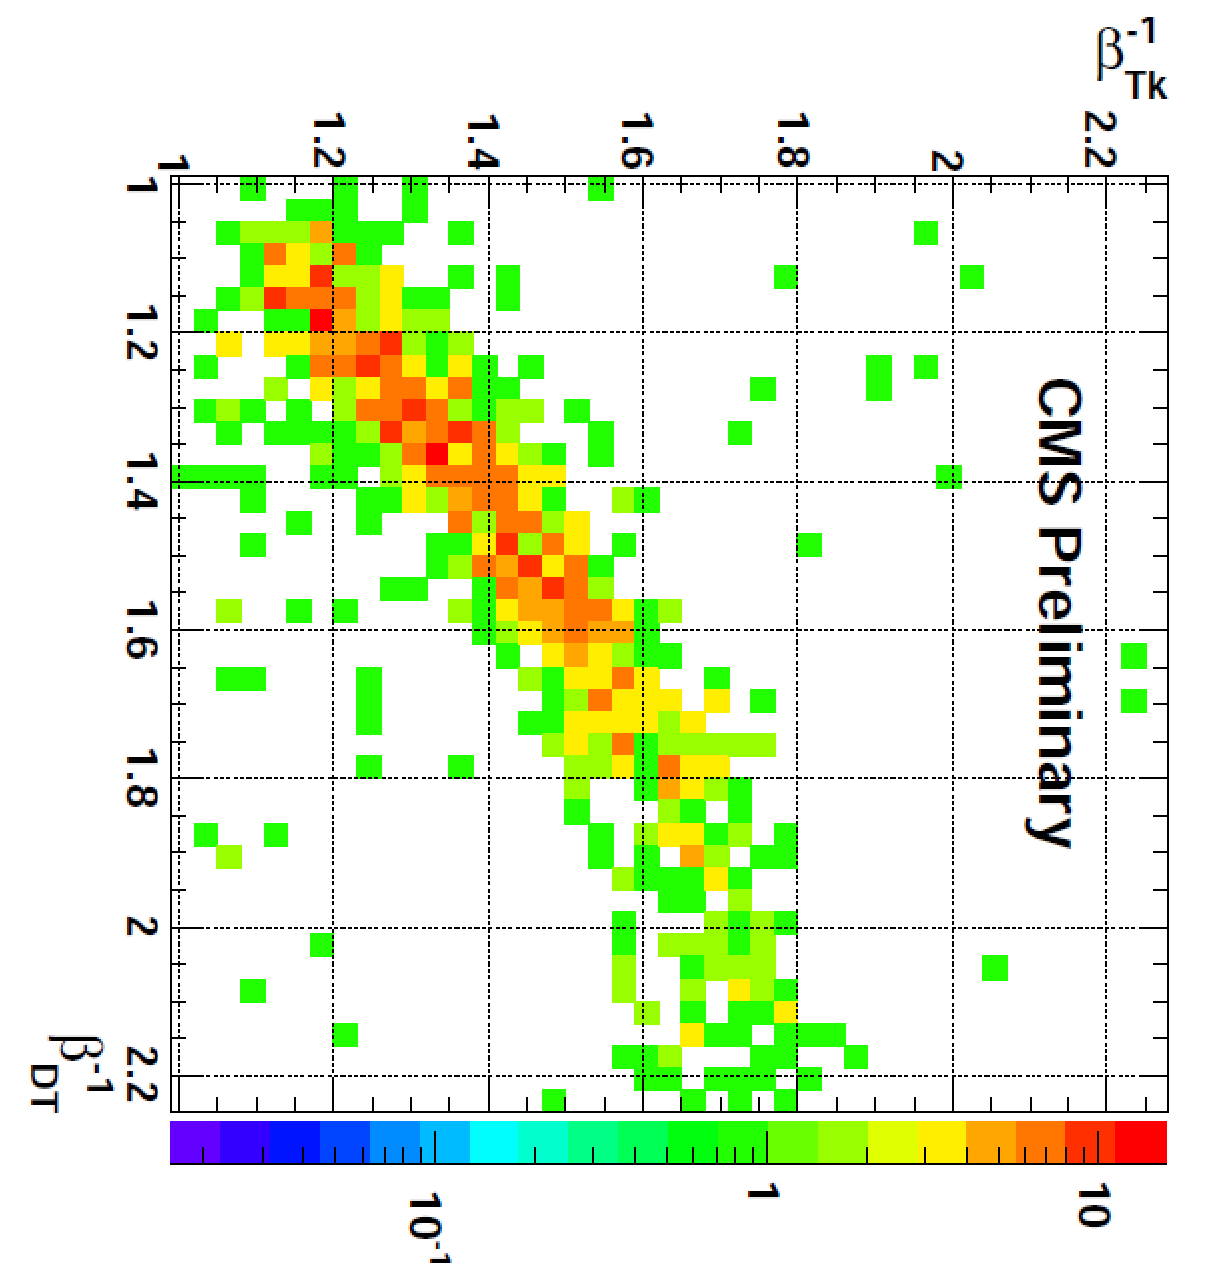
\includegraphics[angle=90,width=0.35\textwidth]{betaHSCPSig.eps}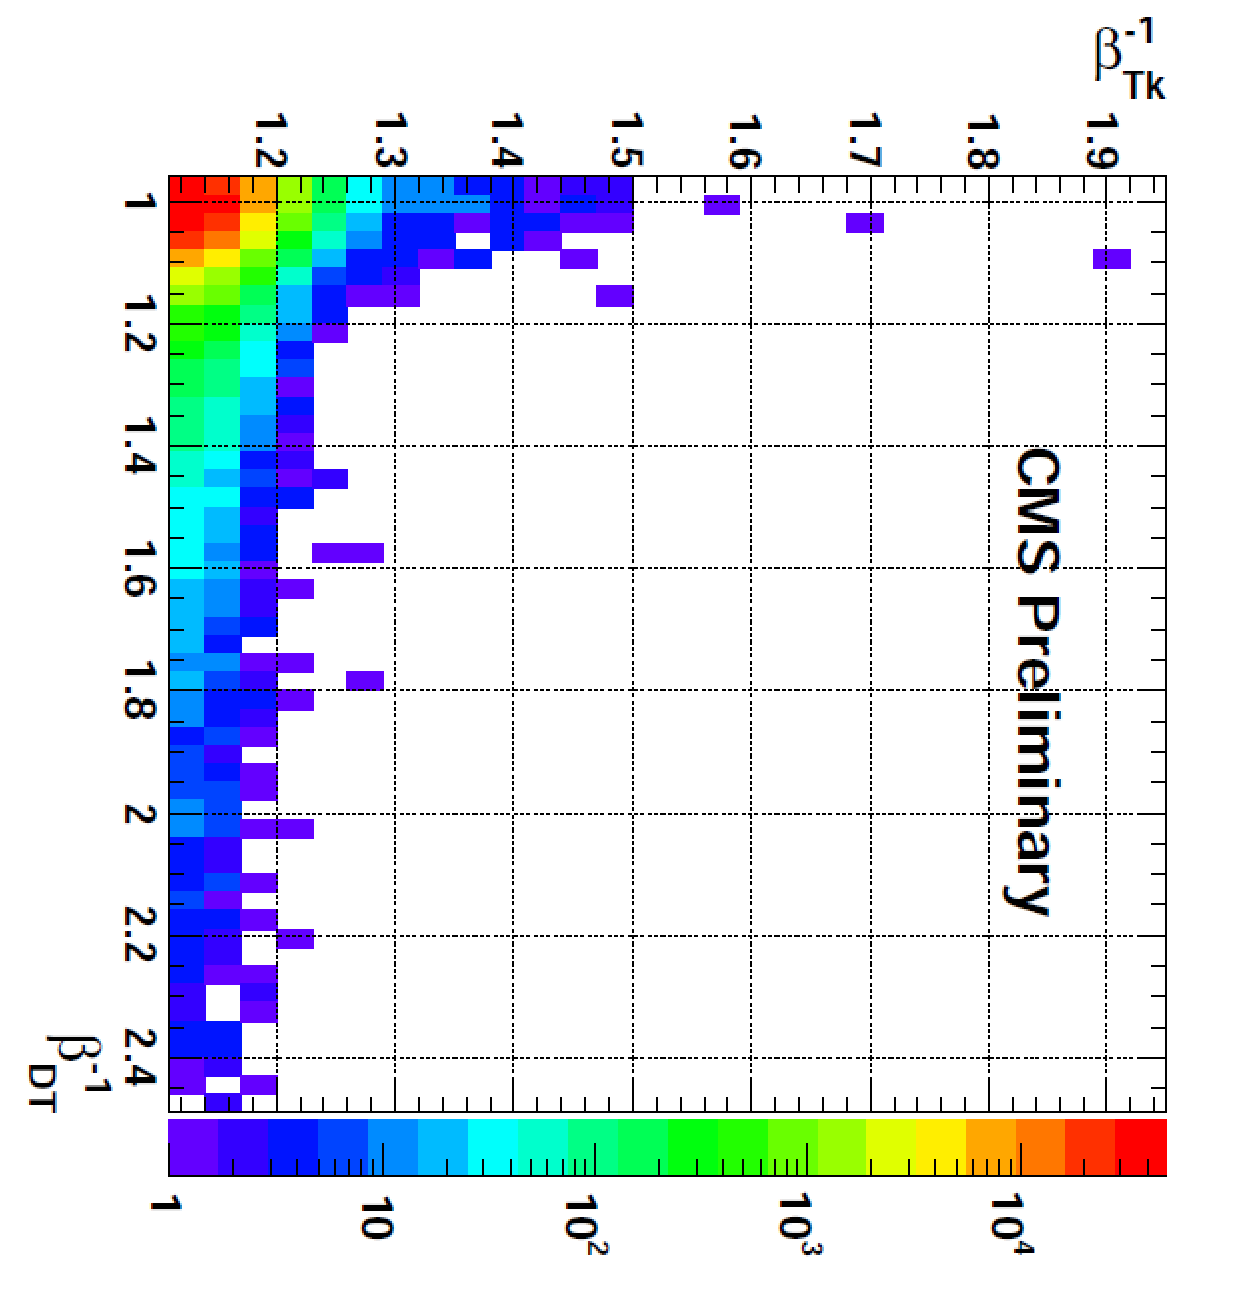
\includegraphics[angle=90,width=0.35\textwidth]{betaHSCPBkg.eps}  
%\caption{Distribution of $\beta_{{\rm Tk}}^{-1}$ {\it vs} $\beta_{{\rm DT}}^{-1}$  
%for signal (stop with mass of 500~GeV/$c^2$) and for SM background (right), 
%for 100~pb$^{-1}$ of data. 
%##Large tails are seen in the background distribution due 
%##to detector resolution and $dE/dx$ statistical fluctuation.
%##The fact that the background mis-measurements of $\beta$ are not correlated  
%##allows to define a region of the plane where signal efficiency is 
%##relatively large and background is almost negligible.
%}
%\label{fig:HSCPSigBkgPlots}
%\end{figure}
%

R-Hadrons lose energy via electromagnetic and nuclear interactions 
while traveling inside the CMS detector. For low-$\beta$ R-hadrons, this energy loss is 
sufficient to bring a significant fraction of the produced particles 
to rest inside the CMS detector volume (in particular in the hadronic calorimeter HCAL). 
These ``stopped'' R-hadrons will decay seconds, day, or weeks later (accordingly to 
the ``unknown'' lifetime). These decays will be out-of-time with respect to the LHC collisions 
and may well occur at times when there are no collisions (e.g., beam gaps) or when there is no beam in 
the LHC machine (e.g., inter-fill period).

For the online selection of these events, the CMS experiment 
developed a dedicated calorimeter trigger. The observation of such decays in a form of an isolated jet 
in HCAL, in what should be a quiet detector (save for the occasional cosmic ray or noise from the 
calorimeters), would be an unambiguous discovery of new physics~\cite{StoppedGluinoPAS}. 
Figure~\ref{fig:StoppedHadron_LQ} (Left) shows 
that few weeks of data taking at $7$~TeV, with an instantaneous luminosity of  $10^{32}$~cm$^{-2}$s$^{-1}$, 
will be sufficient to discover a long-lived gluino of 300~GeV/$c^2$ over a large range of lifetimes.

\begin{figure}[htbp] 
\centering
%eps
%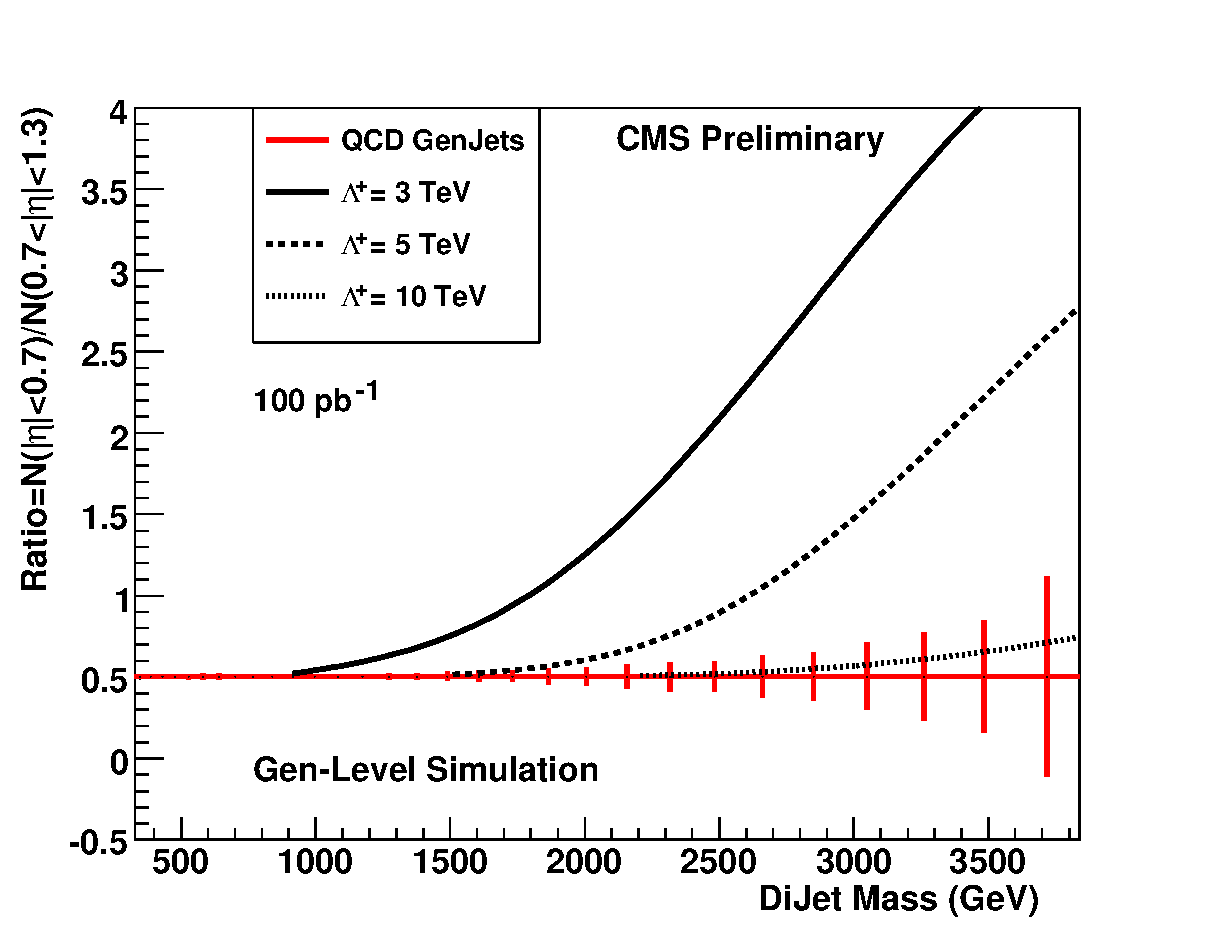
\includegraphics[width=0.5\textwidth]{100pbOptFix.eps}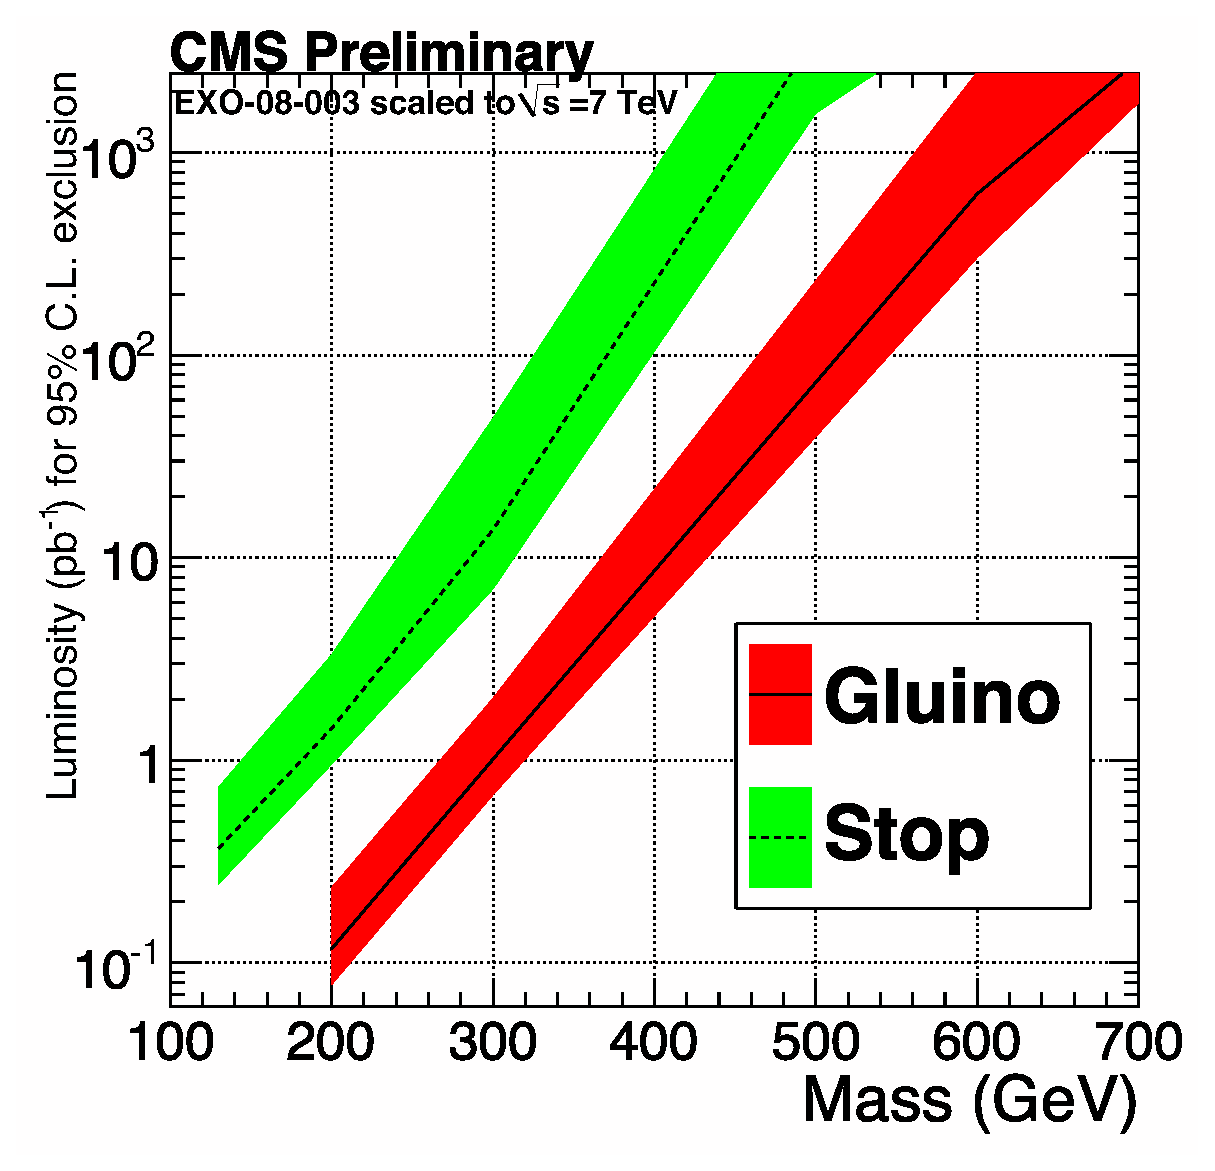
\includegraphics[width=0.4\textwidth]{HSCP1.eps}  
%pdf
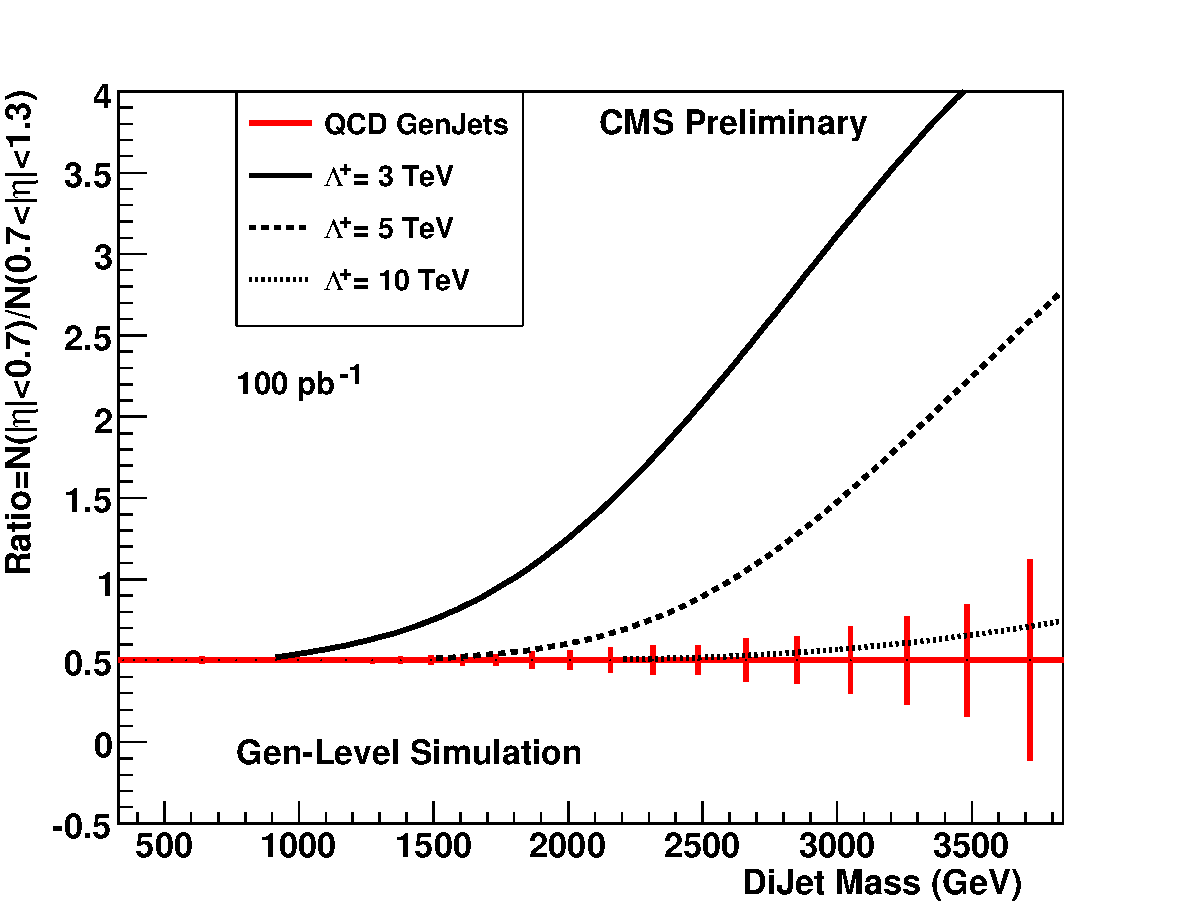
\includegraphics[width=0.5\textwidth]{100pbOptFix.pdf}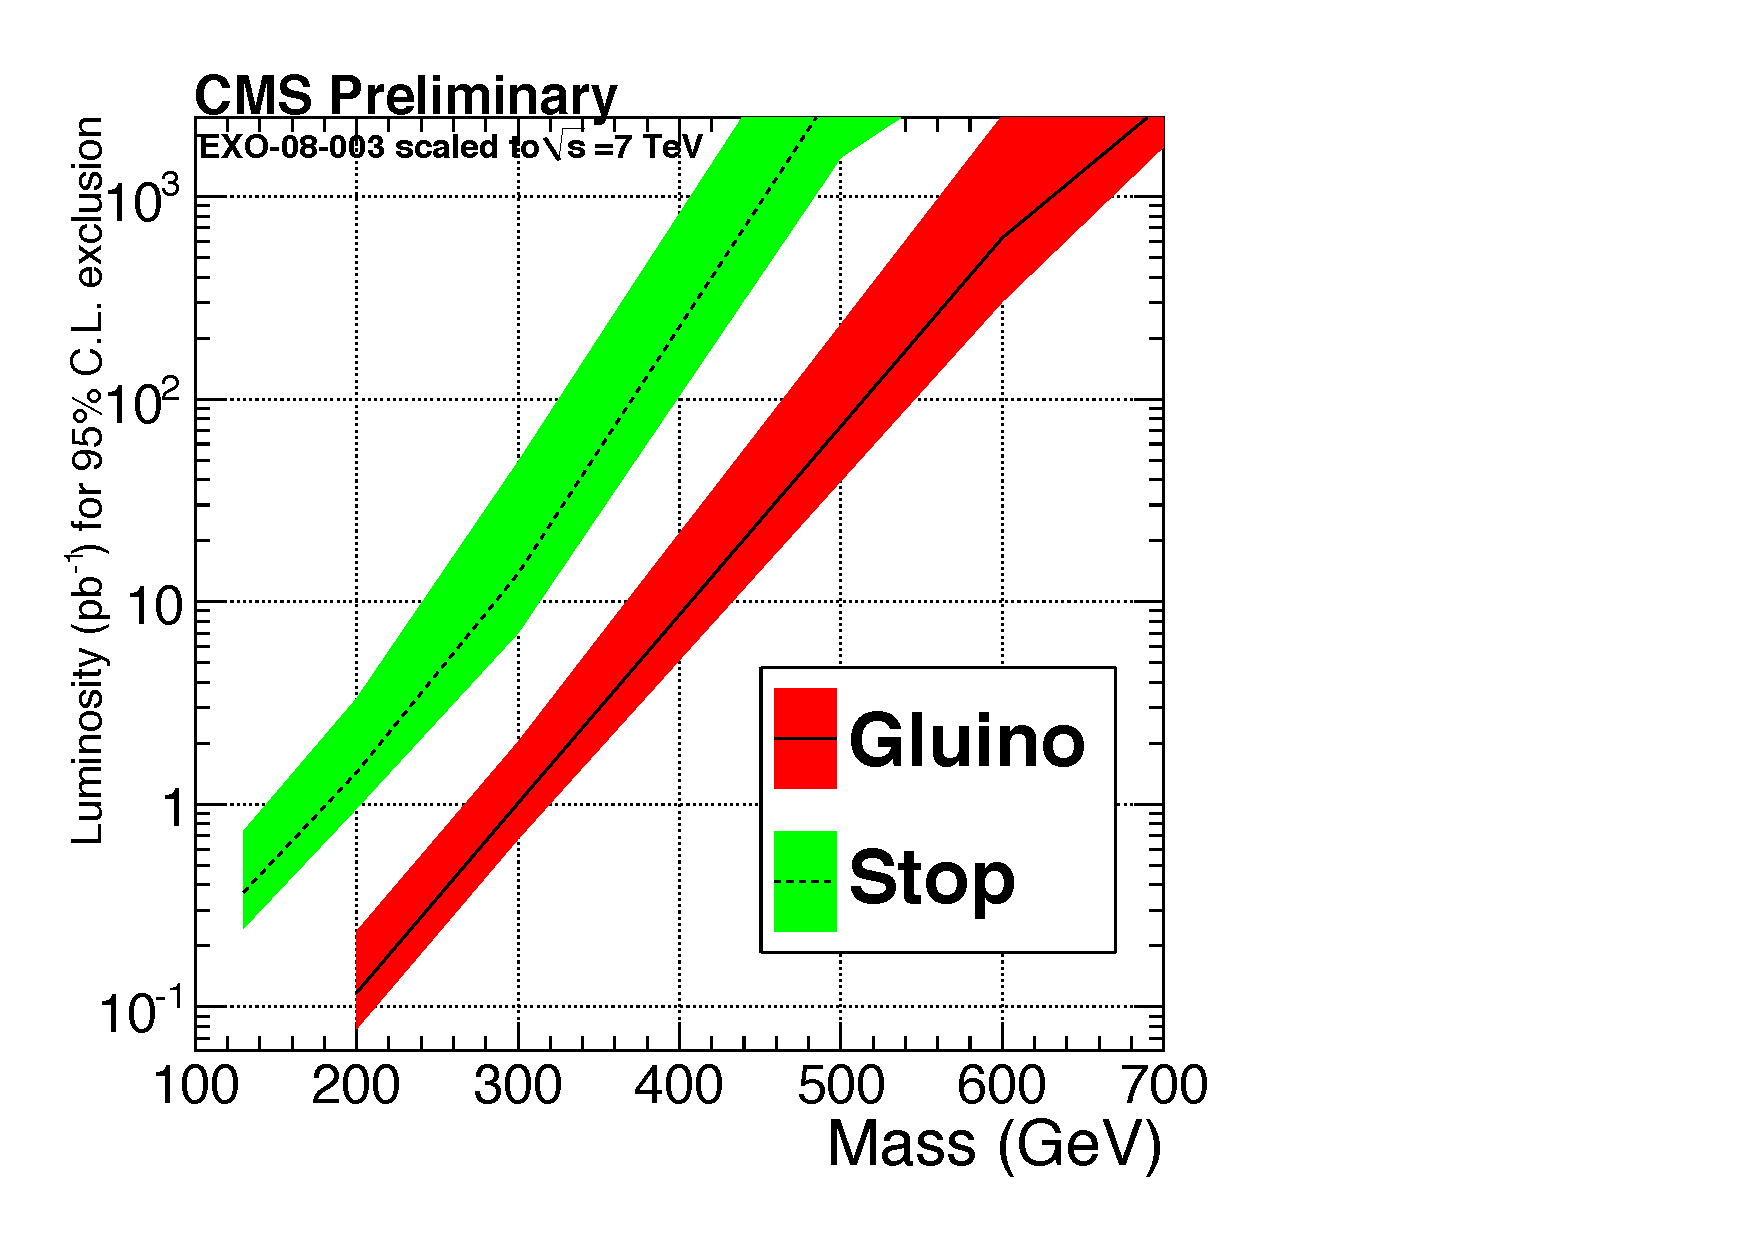
\includegraphics[width=0.4\textwidth]{HSCP1.pdf}  
%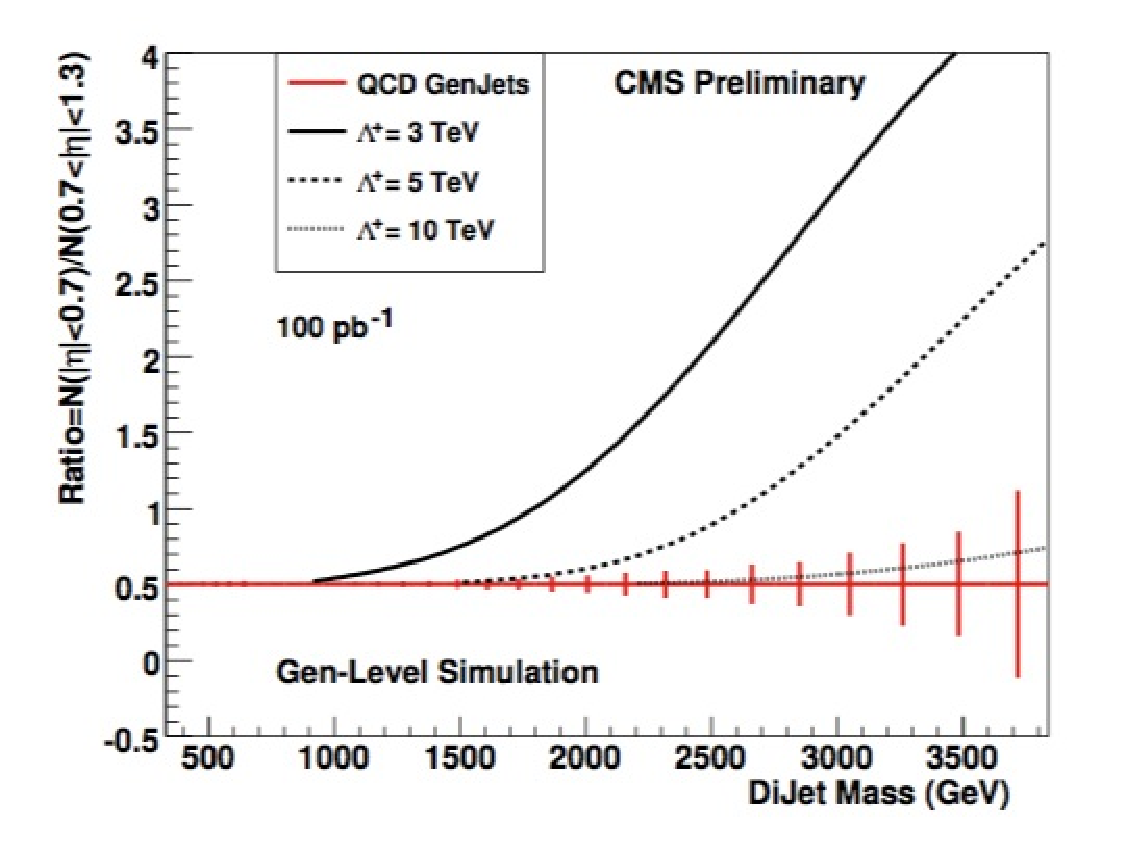
\includegraphics[width=0.5\textwidth]{DiJetRatio100pbOptFix.eps}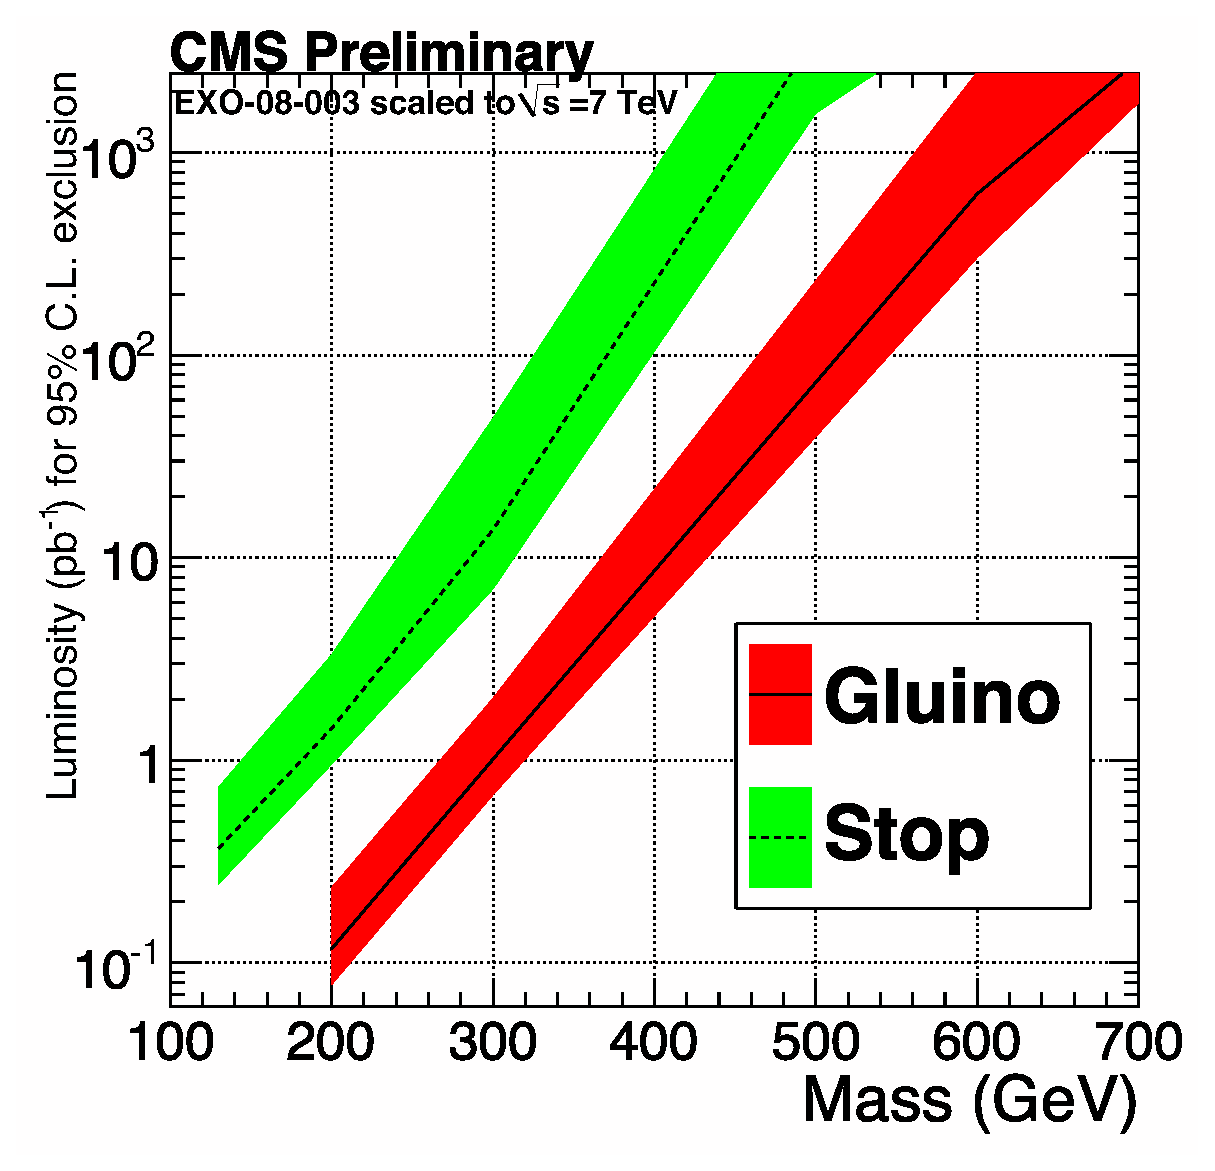
\includegraphics[width=0.4\textwidth]{HSCP1.eps}  
\caption{Left: Di-jet ratio as a function of di-jet mass in presence of 
contact interactions at different energy scales $\Lambda^{+}$, 
and for QCD multi-jet background at $\sqrt{s} = 14$~TeV.  
%For QCD multi-jet events, the di-jet ratio is almost flat at 0.5. 
%In presence of contact interactions, the two 
%leading jets are expected to be more central than in QCD multi-jet events, 
%thus producing a deviation in the di-jet ratio at high di-jet mass values - 
%Right: Di-jet ratio as a function of di-jet mass in presence of 
%exicited quarks at different masses, and for QCD multi-jet background, 
%at $\sqrt{s} = 14$~TeV. 
%Statistical uncertainties on background estimate are reported.  
%Systematics uncertainties, mostly due to jet energy scale, are expected to be small, 
%since significantly reduced in the ratio.
Right: 95\% C.L. limit for HSCP searches at 7 TeV. Tracker-only analysis (i.e. $\beta_{{\rm Tk}}$ measurement) is used. 
Current lower limit of stop mass is around $250$~GeV~\cite{Abazov:2008quETAaltonen:2009kea}.}
\label{fig:DiJetRatioAndHSCP}
\end{figure}


\section{Dilepton+jets channel} \label{leptonjet}
%Some extensions of the SM predict that new physics would manifest itself in 
%final states with high transverse momentum leptons and jets.
%For example, 
The experimentally observed symmetry between families of  
leptons and quarks in the SM has motivated the search for leptoquarks ($LQ$), 
hypothetical bosons carrying both quark and lepton quantum numbers 
that decay in a lepton and a quark.
% ~\cite{Acosta:1999w}.
The pair production of the first (second) generation scalar $LQ$ has been studied in CMS~\cite{LQPAS}, 
in the final state with 2 high $p_T$ electrons (muons) and 2 high $p_T$ jets. 
Figure~\ref{fig:StoppedHadron_LQ} (Right) shows the CMS exclusion reach for the first generation $LQ$ analysis 
with 100~pb$^{-1}$ at $\sqrt{s} = 7$ TeV and the current Tevatron limit. Similar reach is obtained in the $\mu\mu jj$ channel.

\begin{figure}[htbp] 
\centering
%eps
%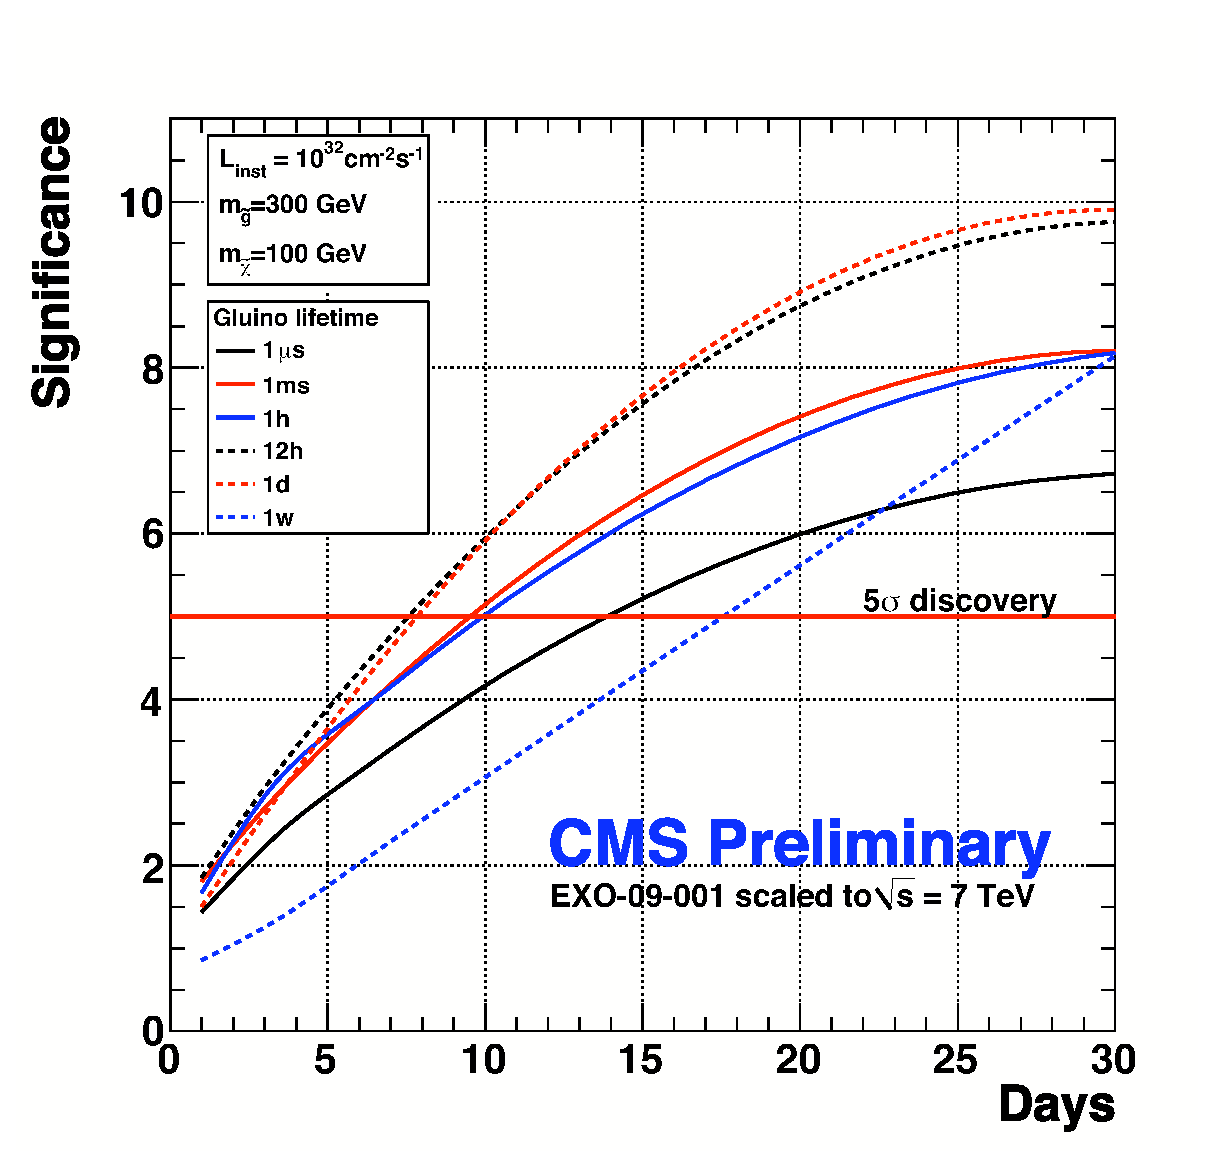
\includegraphics[width=0.4\textwidth]{SG1.eps}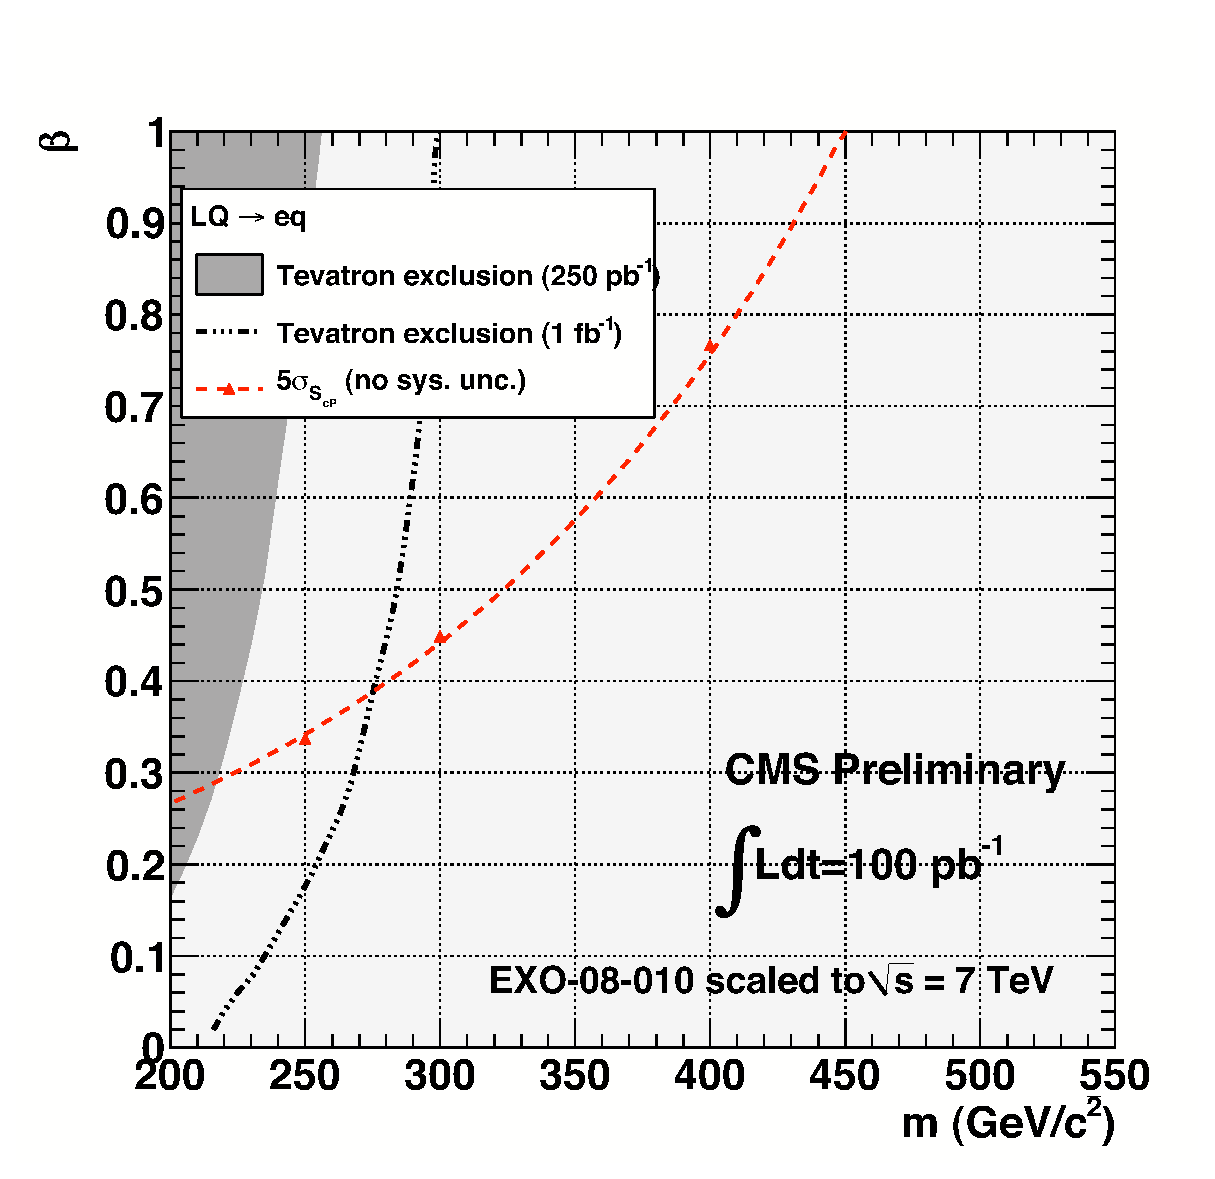
\includegraphics[width=0.4\textwidth]{LQ1.eps}  
%pdf
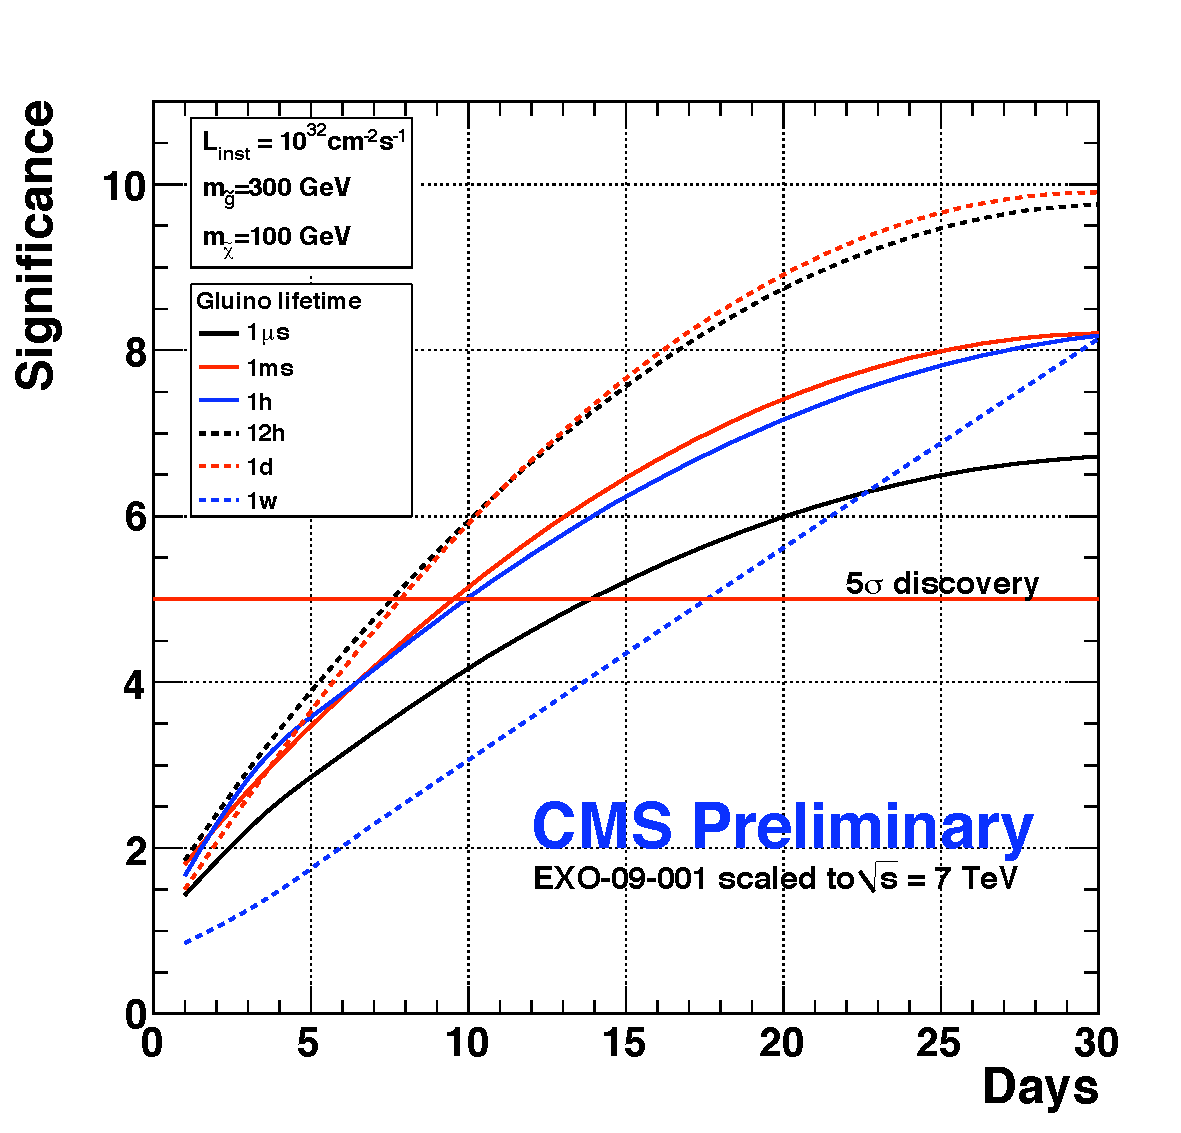
\includegraphics[width=0.4\textwidth]{SG1.pdf}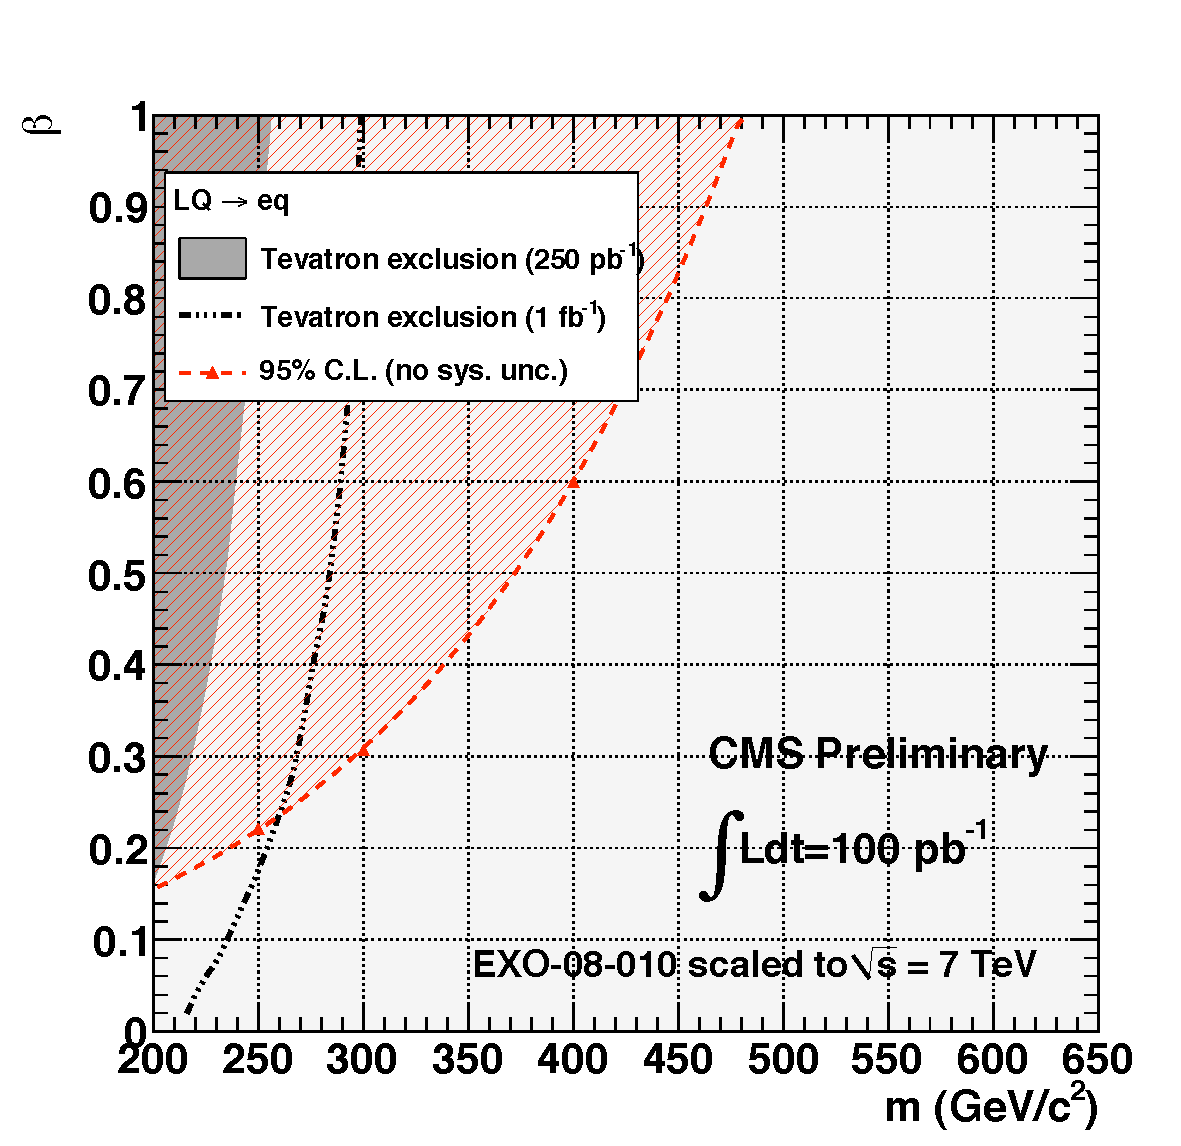
\includegraphics[width=0.4\textwidth]{LQ1_95.pdf}  
\caption{Left: The discovery potential for a long-lived 300~GeV/$c^2$ heavy gluino stopping in the CMS calorimeter 
in a 7 TeV run at an instantaneous luminosity of $10^{32}$~cm$^{-2}$s$^{-1}$ as a function of the data-taking 
duration. Right: The 95\% C.L.limit for first generation leptoquarks in the $ee jj$ channel as 
a function of their branching fraction into electron and quark for 100~pb$^{-1}$ of data at 7 TeV.}
\label{fig:StoppedHadron_LQ}
\end{figure}

\section{Supersymmetry}
CMS will perform a broad range of searches for supersymmetric (SUSY) particles. The initial searches
will be performed in a variety of inclusive final states involving jets, leptons, photons and missing 
transverse energy. Background will be determined using data-driven  methods whenever possible, with multiple 
methods for crosschecks. 

Theorists have noted that the models commonly adopted for use as benchmarks, such as mSUGRA, 
do not span the full range of reasonable phenomenological patterns for which experiments should search.
As a consequence, it is important to design searches that are as generic as possible.
Nevertheless, the sensitivity of the analyses for 100~pb$^{-1}$ and 1~fb$^{-1}$ 
at $7$~TeV~\cite{CMSPhysicsReach7TeV} is presented in Figure~\ref{fig:SUSY} 
, for both all-hadronic and like-sign dilepton signatures, using a scan over mSUGRA parameters,  
since it allows direct comparison with existing results from Tevatron and LEP experiments.

\begin{figure}[htbp] 
\centering
%eps
%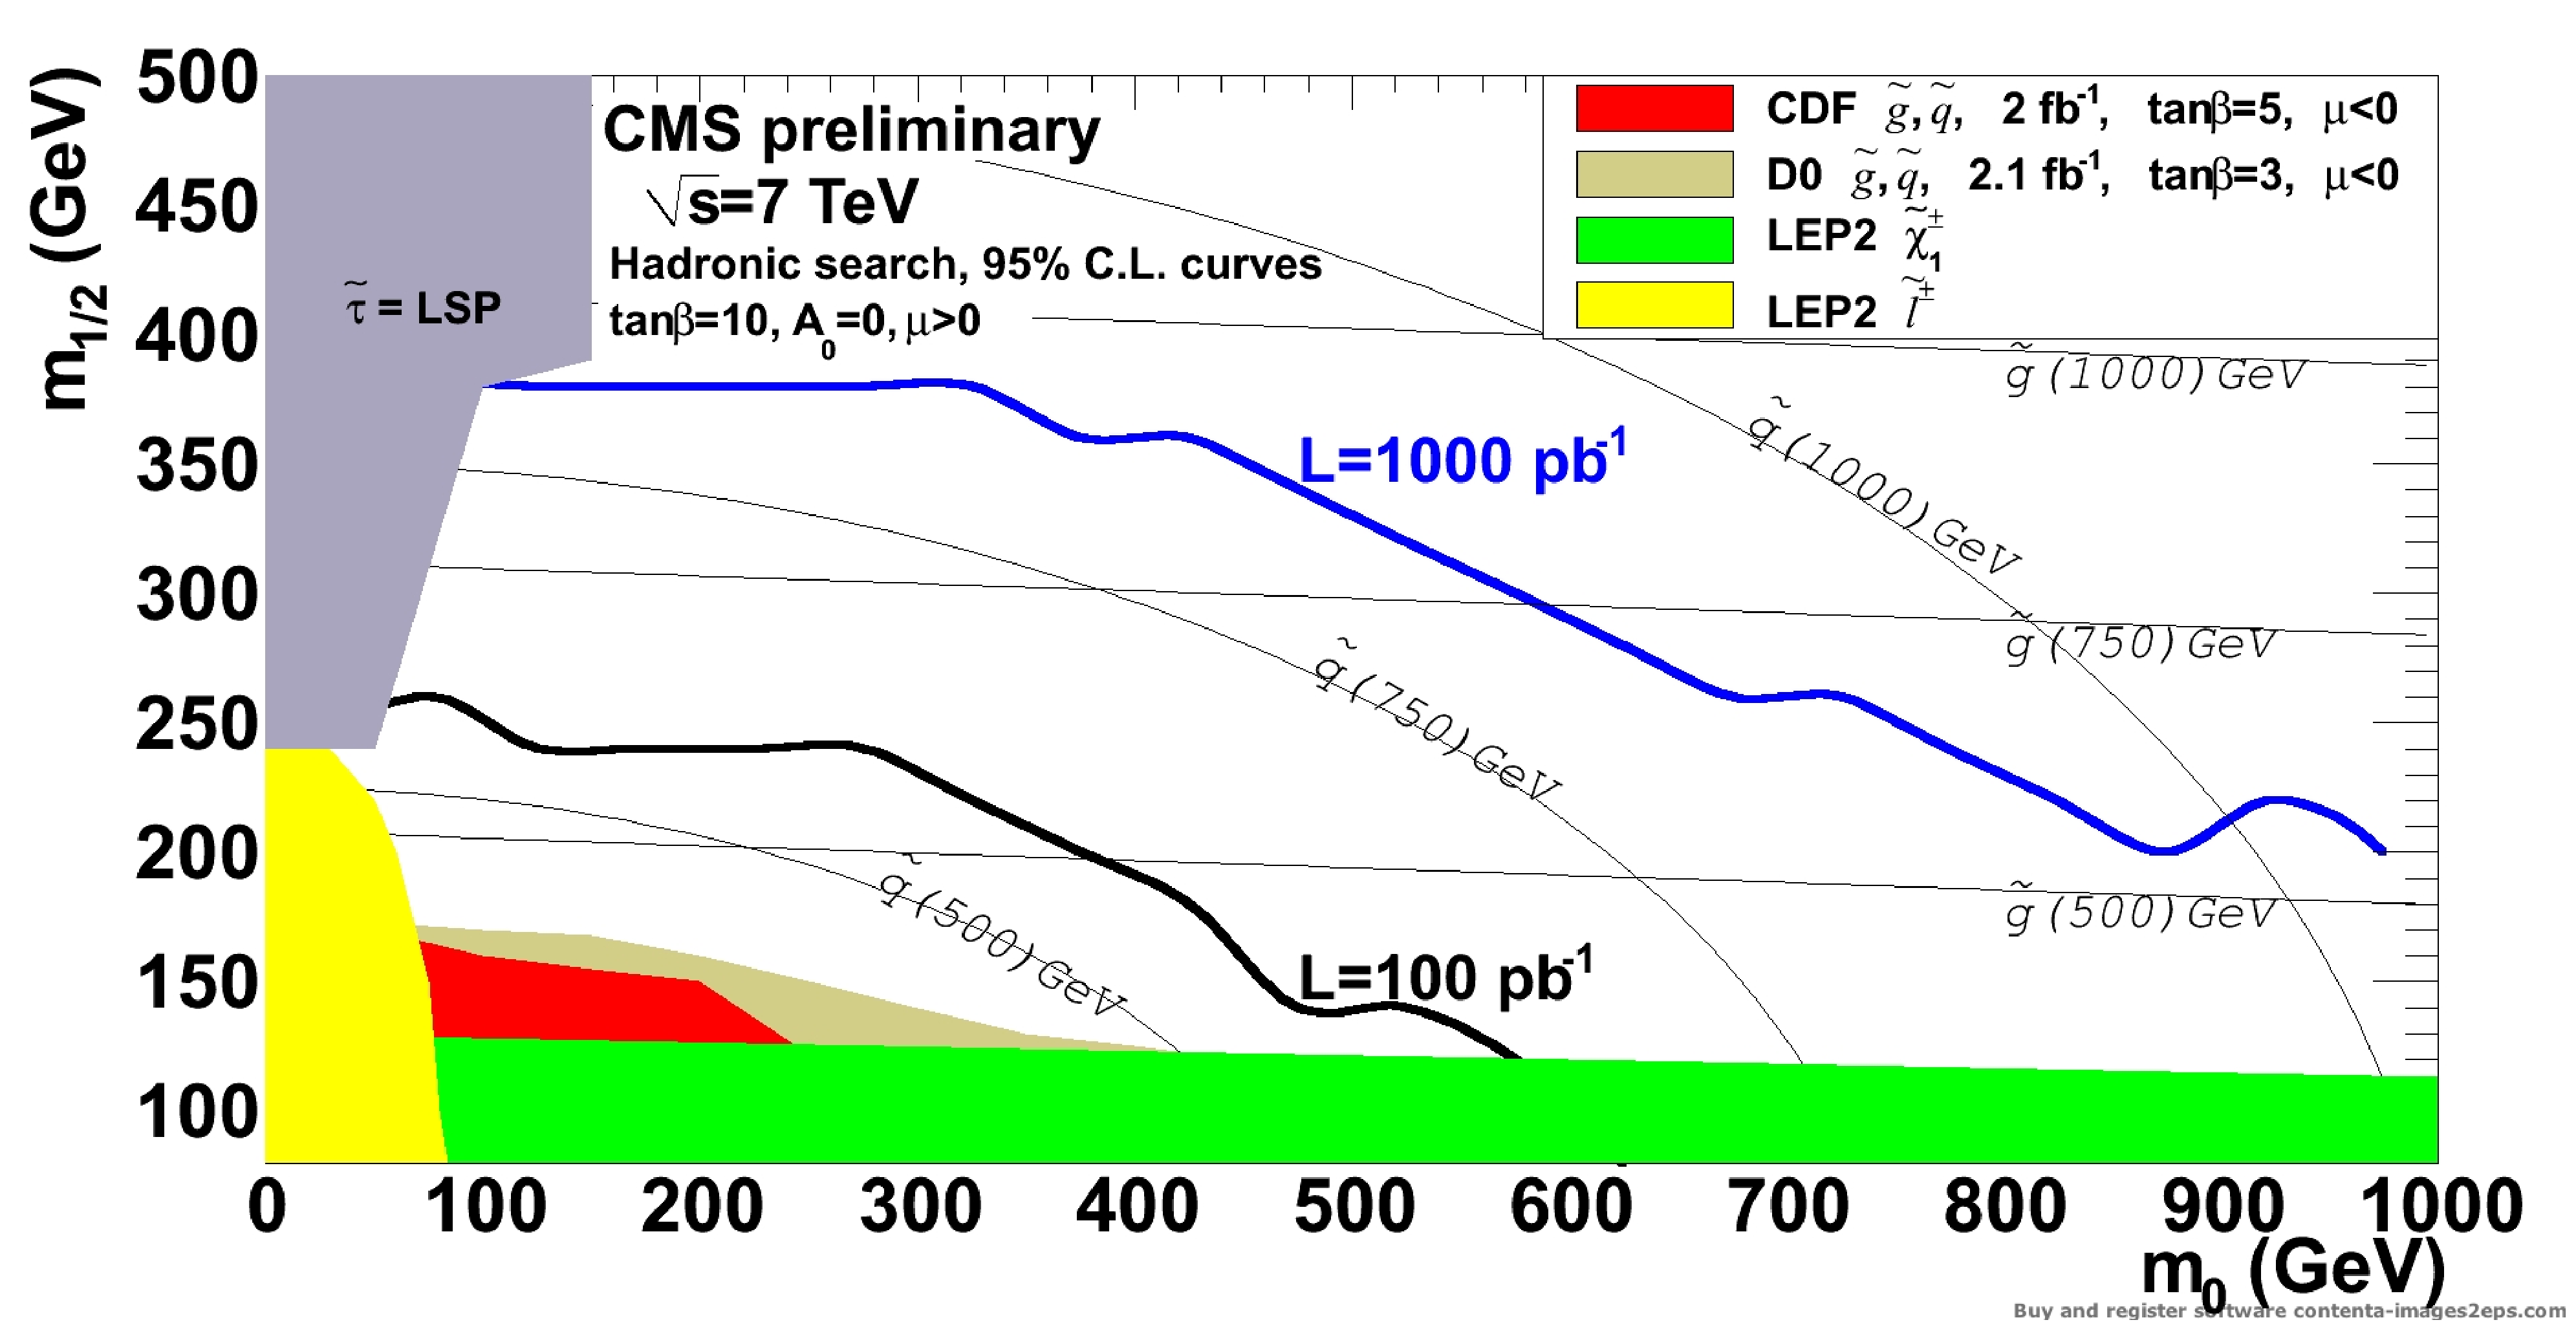
\includegraphics[width=0.6\textwidth]{SUSY_Fig1.eps}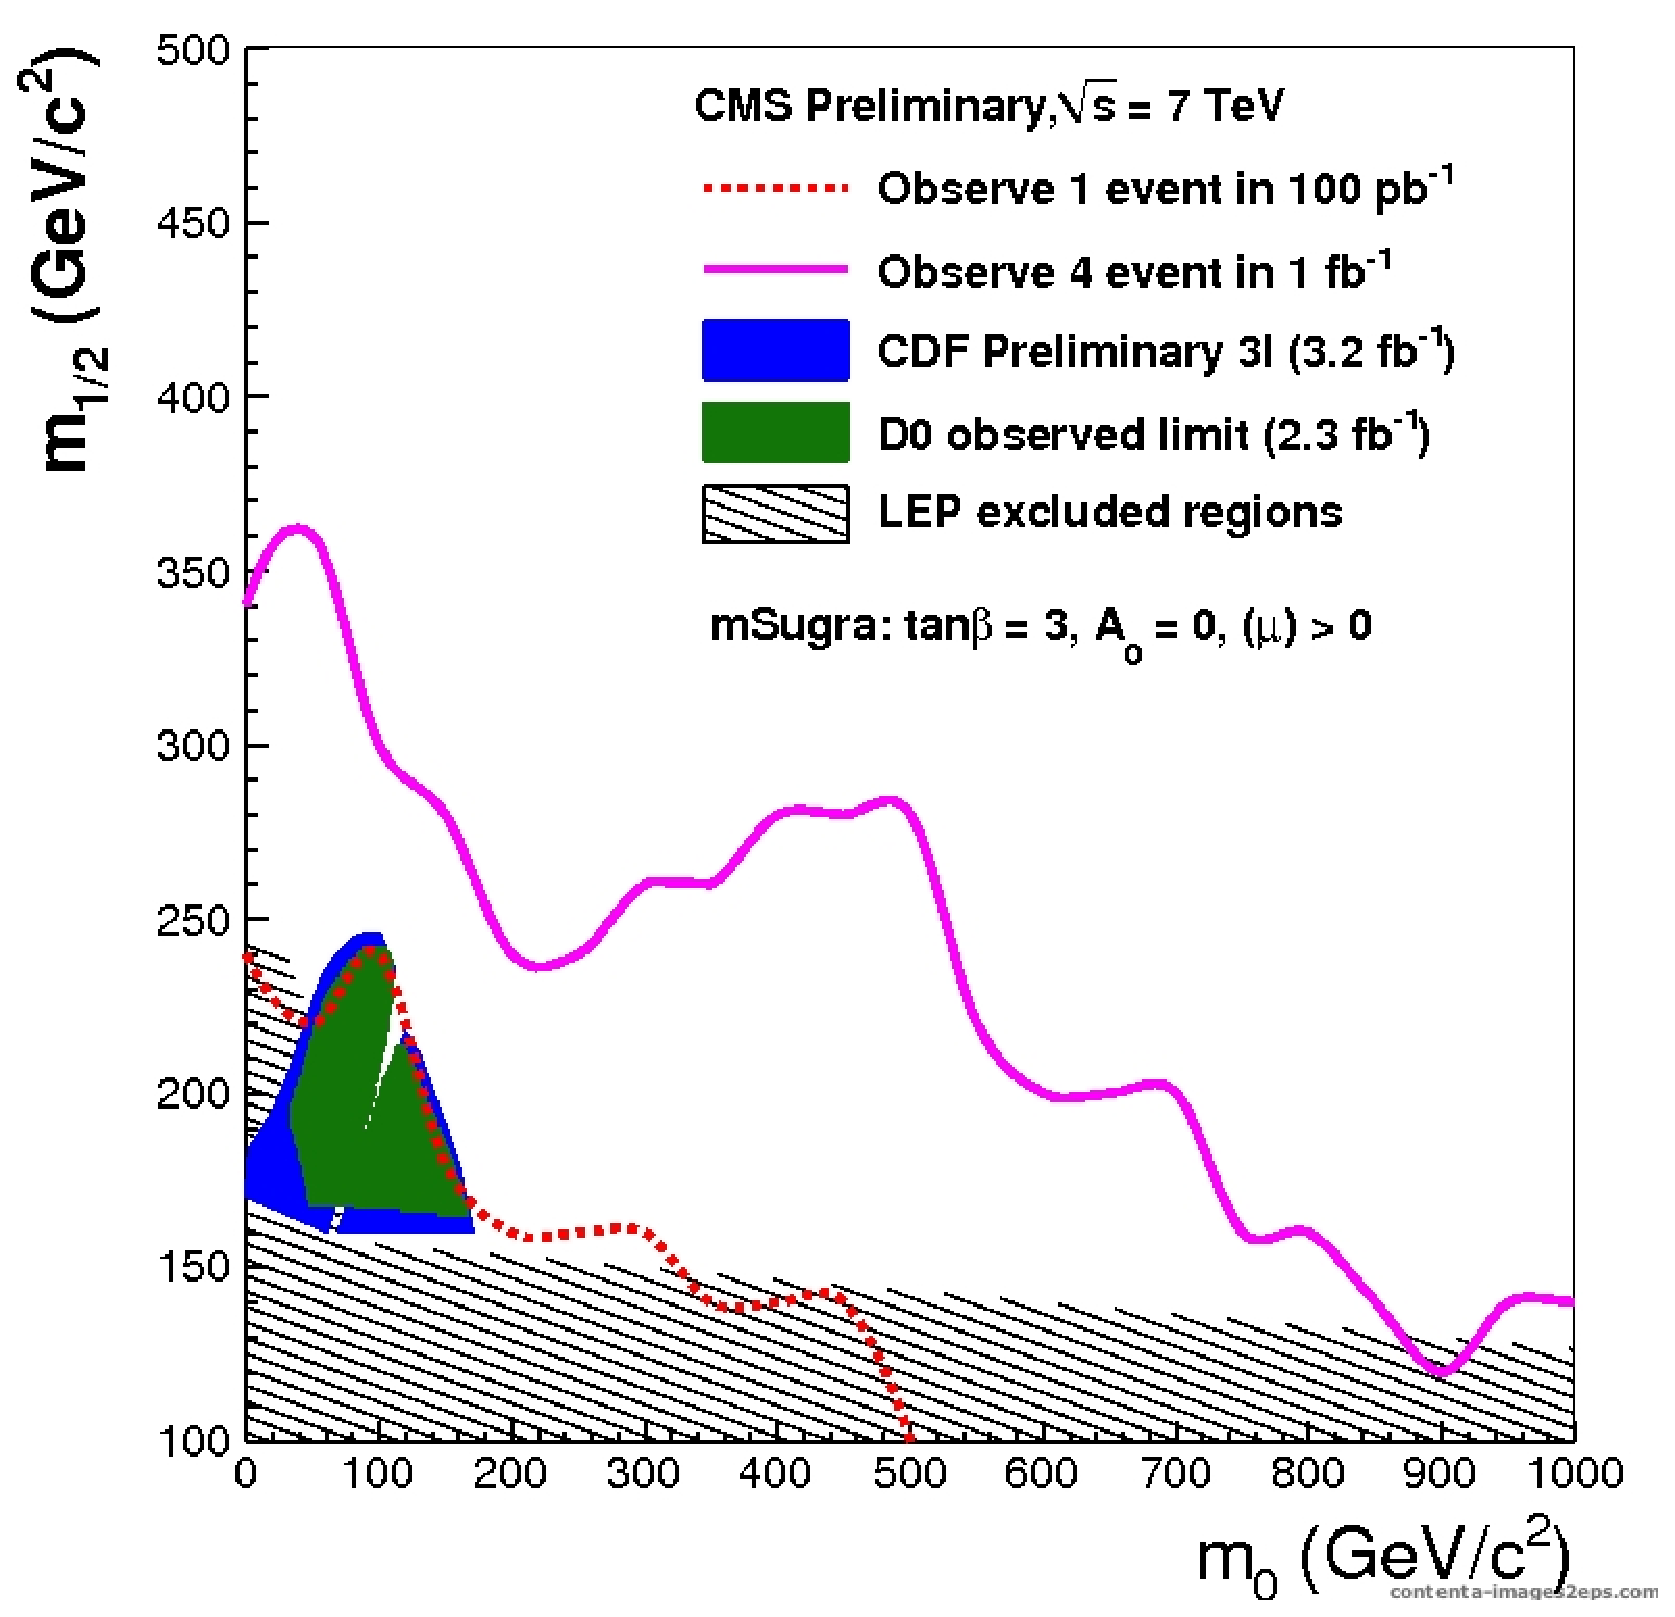
\includegraphics[width=0.4\textwidth]{SUSY_Fig2.eps}  
%jpg
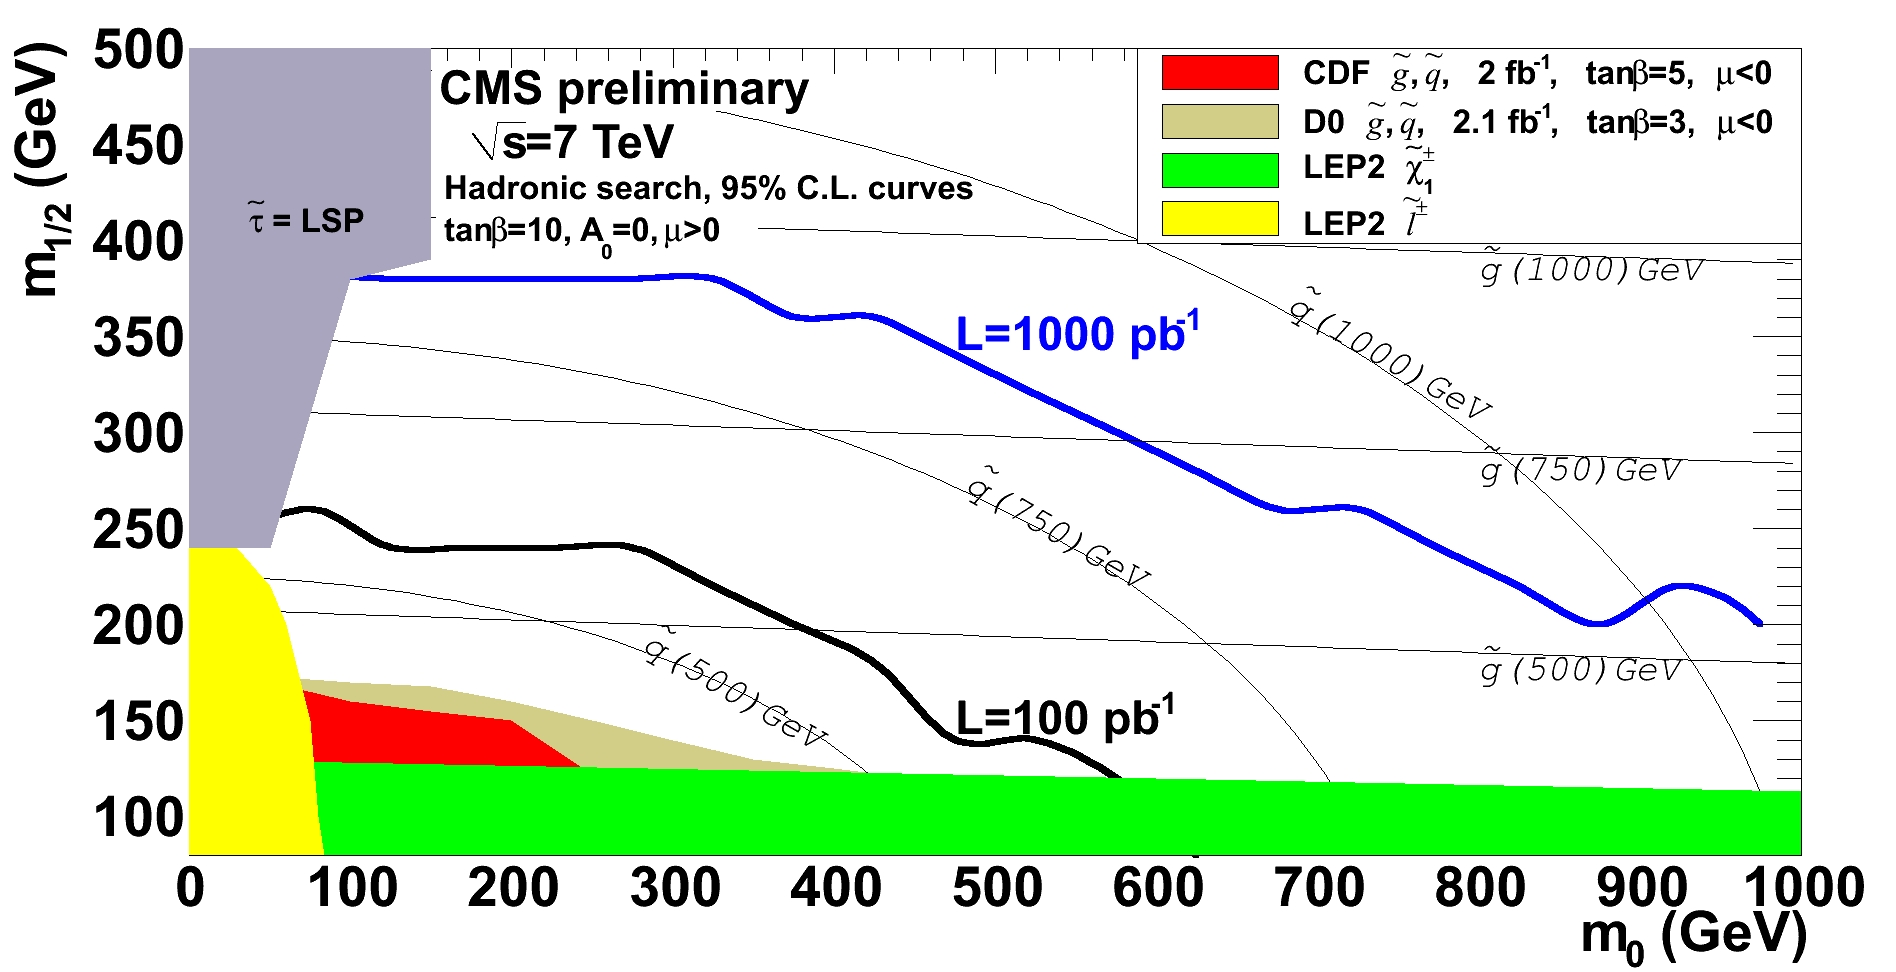
\includegraphics[width=0.6\textwidth]{SUSY_Fig1.jpg}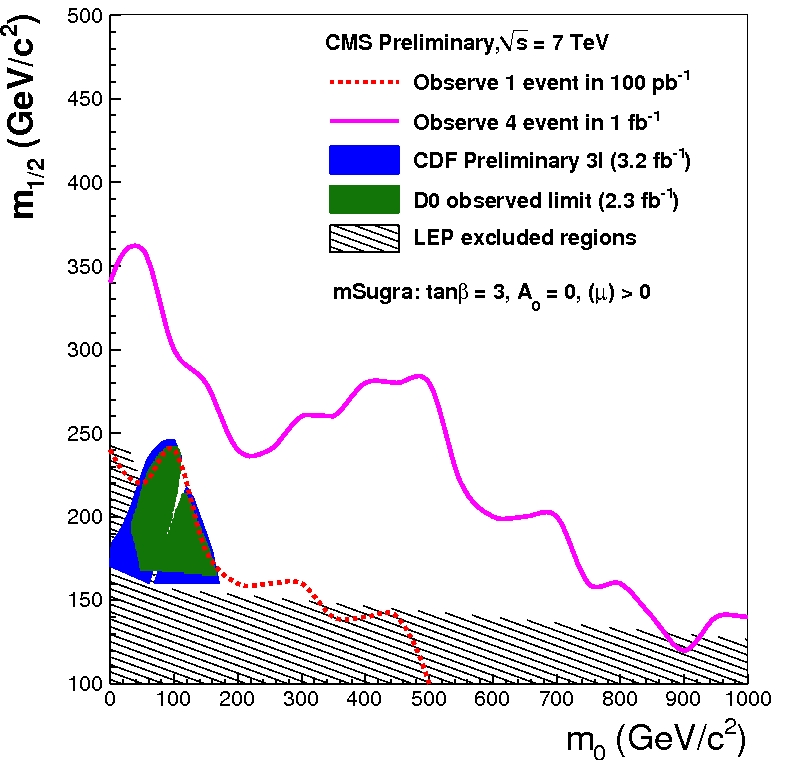
\includegraphics[width=0.4\textwidth]{SUSY_Fig2.jpg}  
\caption{Left: Estimated 95\% C.L. exclusion limits for the all-hadronic SUSY search, expressed in mSUGRA 
parameter space. Right: Estimated 95\% C.L. exclusion limits for the like-sign dilepton SUSY search, 
expressed in mSUGRA parameter space. The expected standard model background at 100~pb$^{-1}$ (1~fb$^{-1}$) 
is 0.4 (4.0) events; an observed yield of 1 event (4 events) is assumed for the purpose of setting these exclusion limits.}
\label{fig:SUSY}
\end{figure}

\section{Conclusions}
At the time of the conference (April 2010), the LHC delivered a fraction of nb$^{-1}$ 
of pp collisions at $\sqrt{s} = 7$~TeV. 
%The current expectation 
%is to collect order of 100~nb$^{-1}$ of data by the middle of July, just before 
%the ICHEP summer conference. 
This amount of integrated luminosity is not  
sufficient to improve the existing constrains on new physics set by other experiments; 
anyway, for some of the analyses presented here, this ``turning point'' could 
already be reached with 1 - 10~pb$^{-1}$ of data.

The LHC is expected to deliver approximately 100~pb$^{-1}$ of integrated luminosity 
between the end of 2010 and the beginning of 2011, and 1~fb$^{-1}$ by the end of 2011. 
This large $7$~TeV dataset will allow to set stringent limits 
on many exotic theoretical models, and, if Nature is kind to us, 
to even observe the first evidence of new physics beyond the SM.

\begin{thebibliography}{0}
%%%%%%%%%%
%%%%%%%%%%
%\cite{CMS:2008zzk}
\bibitem{CMS:2008zzk}
  R.~Adolphi {\it et al.}  [CMS Collaboration],
  ``The CMS experiment at the CERN LHC,''
  JINST {\bf 3}, S08004 (2008).
  %%CITATION = JINST,3,S08004;%%
%@Article{Bayatian:2006zz,
%     author    = ``Bayatian, G. L. and others'',
% collaboration = ``CMS'',
%     title     = ``{CMS physics: Technical design report}'',
%     note     = ``CERN-LHCC-2006-001''
%}
%\cite{Bayatian:2006zz}
%\bibitem{Bayatian:2006zz}
%  G.~L.~Bayatian {\it et al.}  [CMS Collaboration],
%  ``CMS physics: Technical design report''
%  %%CITATION = CMS-TDR-008-1;%%
% \quad
% G.~L.~Bayatian {\it et al.}  [CMS Collaboration],
% ``CMS technical design report, volume II: Physics performance,''
% J.\ Phys.\ G {\bf 34} (2007) 995.
% %%CITATION = JPHGB,G34,995;%%
\bibitem{CMSPhysicsReach7TeV}
  CMS Collaboration,
  ``The CMS physics reach for searches at 7 TeV,''
  CMS-NOTE-2010-008 (2010).
%@techreport{Collaboration:1264099,
%      author       = ``CMS Collaboration'',
%      title        = 
%      institution  = ``CERN'',
%      address      = ``Geneva'',
%      number       = ``CMS-NOTE-2010-008. CERN-CMS-NOTE-2010-008'',
%      month        = ``May'',
%      year         = ``2010'',
%}
%\bibitem{Baur:1989kv}
%  U.~Baur, M.~Spira and P.~M.~Zerwas,
%  ``EXCITED QUARK AND LEPTON PRODUCTION AT HADRON COLLIDERS,''
%  Phys.\ Rev.\  D {\bf 42}, 815 (1990).
%  %%CITATION = PHRVA,D42,815;%%
%\bibitem{Bagger:1987fz}
%  J.~Bagger, C.~Schmidt and S.~King,
%  ``AXIGLUON PRODUCTION IN HADRONIC COLLISIONS,''
%  Phys.\ Rev.\  D {\bf 37}, 1188 (1988).
%  %%CITATION = PHRVA,D37,1188;%%
%\bibitem{Angelopoulos:1986uq}
%  V.~D.~Angelopoulos, J.~R.~Ellis, H.~Kowalski, D.~V.~Nanopoulos, N.~D.~Tracas and F.~Zwirner,
%  %``SEARCH FOR NEW QUARKS SUGGESTED BY THE SUPERSTRING,''
%  Nucl.\ Phys.\  B {\bf 292}, 59 (1987).
%  %%CITATION = NUPHA,B292,59;%%
%\bibitem{Eichten:1983hw}
%  E.~Eichten, K.~D.~Lane and M.~E.~Peskin,
%  ``New Tests For Quark And Lepton Substructure,''
%  Phys.\ Rev.\ Lett.\  {\bf 50}, 811 (1983).
%  %%CITATION = PRLTA,50,811;%%
\bibitem{DIJETSNOTE}
 CMS Collaboration,
 ``CMS Search Plans and Sensitivity to New Physics using Dijets,''
 CMS-PAS-SBM-07-001 (2007), and references on the theory therein.
\bibitem{Abbott:1998wh}
  B.~Abbott {\it et al.}  [D0 Collaboration],
  %``The dijet mass spectrum and a search for quark compositeness in $\bar{p}p$
  %collisions at $\sqrt{s} = 1.8$ TeV,''
  Phys.\ Rev.\ Lett.\  {\bf 82}, 2457 (1999)
  [arXiv:hep-ex/9807014].
  %%CITATION = PRLTA,82,2457;%%
\bibitem{Fairbairn:2006gg}
  M.~Fairbairn, A.~C.~Kraan, D.~A.~Milstead, T.~Sjostrand, P.~Z.~Skands and T.~Sloan,
  ``Stable massive particles at colliders,''
  Phys.\ Rept.\  {\bf 438}, 1 (2007)
  [arXiv:hep-ph/0611040].
  %%CITATION = PRPLC,438,1;%%
\bibitem{HSCP}
 CMS Collaboration,
 ``Search for Heavy Stable Charged Particles with 100 inverse picobarns and 1 inverse femtobarn in the CMS experiment,''
 CMS-PAS-EXO-08-003 (2009)
\bibitem{TRACKERPAS}
 CMS Collaboration,
 ``Tracking and Vertexing Results from First Collisions,''
 CMS-PAS-TRK-10-001 (2009).
\bibitem{StoppedGluinoPAS}
  CMS Collaboration,
  ``Searching for Stopped Gluinos during Beam-off Periods at CMS,''
  CMS-PAS-EXO-09-001 (2009)
\bibitem{Abazov:2008quETAaltonen:2009kea}
  V.~M.~Abazov {\it et al.}  [D0 Collaboration],
  ``Search for Long-Lived Charged Massive Particles with the D0 Detector,''
  Phys.\ Rev.\ Lett.\  {\bf 102}, 161802 (2009)
  [arXiv:0809.4472 [hep-ex]].
  %%CITATION = PRLTA,102,161802;%%
\quad
  T.~Aaltonen {\it et al.}  [CDF Collaboration],
  ``Search for Long-Lived Massive Charged Particles in 1.96 TeV $\bar{p}p$ Collisions,''
  Phys.\ Rev.\ Lett.\  {\bf 103}, 021802 (2009)
  [arXiv:0902.1266 [hep-ex]].
  %%CITATION = PRLTA,103,021802;%%  
\bibitem{LQPAS}
  CMS Collaboration,
  ``Search for Pair Production of First Generation Scalar Leptoquarks at the CMS Experiment,''
  CMS-PAS-EXO-08-010 (2009)
\quad 
  CMS Collaboration,
  ``Search for Second Generation Scalar Leptoquarks with the CMS Detector,''
  CMS-PAS-EXO-09-010 (2009), and references on the model therein.
\end{thebibliography}

\end{document}
